\section{Detektionsmetoder}
Der er mange måder at detektere exoplaneter på, men fælles for dem alle er, at de involverer lys fra enten planeten selv eller en anden lyskilde. At opdage planeter kræver derfor en forståelse af lys, hvordan det opstår og påvirkes af sine omgivelser. Det er dog muligt at få en god forståelse af de fysiske fænomener, der ligger til grund for disse metoder, uden en dybdegående forståelse af de teorier, der detaljeret beskriver fænomenerne. Eksempelvis kan gravitationslinsemetoden, som beskrevet senere, sagtens forstås overfladisk uden kendskab til generel relativitetsteori, hvis man er villig til at acceptere, at lys er påvirket af tyngdekraften analogt til objekter med masse. Formålet med dette afsnit er derfor at give en fænomenologisk og forhåbentlig intuitiv forståelse af, hvordan vi mennesker på Jorden kan opdage planeter uden for Solsystemet.\footnote{Til dette formål kan der med fordel henvises til nogle særdeles glimerende animationer på \url{https://exoplanets.nasa.gov/5-ways-to-find-a-planet/}.}

\subsection*{Direkte observation}

Den mest nærliggende metode er nok at pege sit teleskop mod et stjernesystem, og direkte se om noget ligner en planet. Dette er dog svært i praksis. Problemet er at exoplaneter fylder meget lidt på himlen, når de er så langt væk, så den eneste måde vi ville kunne se dem, var hvis de lyste. Men det er faktisk muligt. For hvis vi kigger i den infrarøde del af spektret, så lyser Solen fx kun 100 gange mere end Jupiter. %For når en stjerne lyser på en planet, kan planeten reflektere en del af lyset, og på den måde kan vi se den. 
Men hvilke planeter er så lettest at se? \\
Svaret er, at jo større en planet er, des mere lys vil den udsende. Derfor er planeterne detekteret ved direkte observation så store, at de er på grænsen til at være brune dværgstjerner. %reflekterer mere lys jo tættere den er på stjernen (der er mere lys at reflektere) og jo større den er (større planetoverflade til at reflektere lyset). Man kunne måske tænke planetens farve også har noget at sige, men denne effekt er meget mindre. %citation needed
%
%Indsæt formel
%
Lysstyrken bliver dog aldrig særlig høj sammenlignet med stjerner. Og ligesom alt andet lys, aftager fluxen her som $F\propto D^{-2}$ ifølge afstandskvadratloven i ligning \eqref{afstandskv}. Dette betyder at metoden kun virker for gaskæmper, der kredser meget langt fra deres stjerner. Store planeter lyser mere, og afstanden gør at lyset kan skelnes fra stjernens. Vi kan kun se dem der kredser om stjerner tæt på vores eget solsystem, så fluxen ikke er faldet for meget med afstanden. %varme jupita? Jupitorer?
%
Et eksempel på planeter opdaget ved direkte observation, er dem om stjernen HR 8799 på figur \ref{DI}. Her har man blokeret selve stjernens lys, så det ikke blænder for den smule infrarødt lys, vi modtager fra planeterne omkring den.

\begin{figure}[h!]
    \centering
    \begin{subfigure}{.45\textwidth}
        \centering
        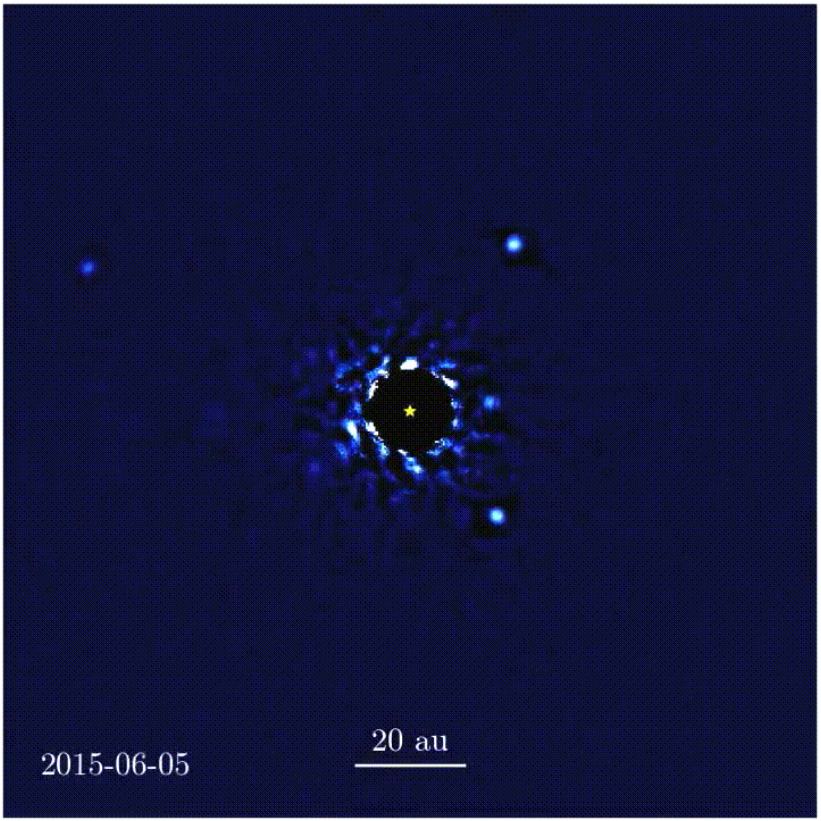
\includegraphics[width = 0.95\textwidth]{Astrofysik/billeder/Direct_imaging_image.PNG} 
        \caption{Direkte observation af mindst 4 store exoplaneter om stjernen HR 8799. AU står for astronomical unit og er afstanden fra Jorden til Solen. Til sammenligning er Jupiter 5 AU fra Solen.}
        \label{DI}
    \end{subfigure}
    \hspace{5mm}
    \begin{subfigure}{.45\textwidth}
        \centering
        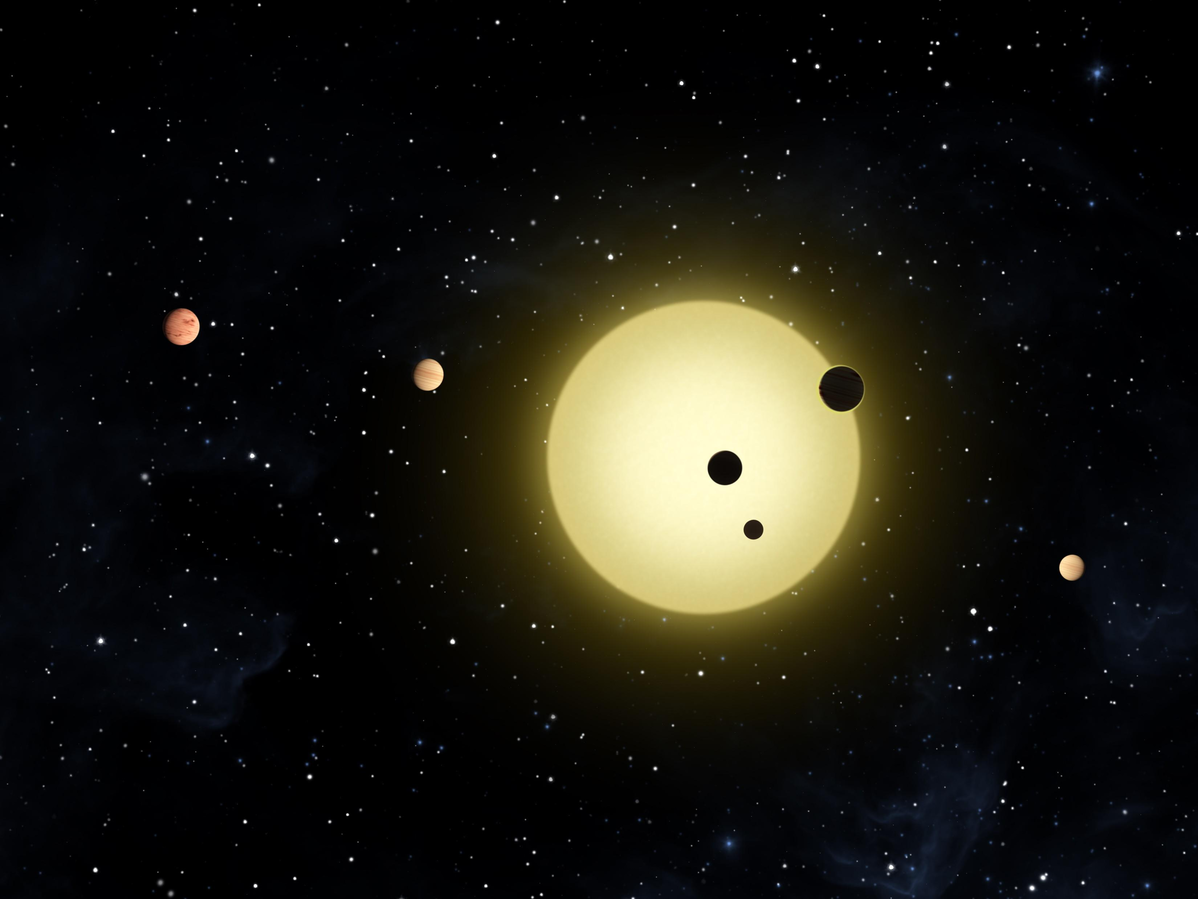
\includegraphics[width = 0.95\textwidth]{Astrofysik/billeder/Kepler11.png} 
        \caption{Kunstnerisk afbildning af stjernen Kepler 11 med planeter i transit.}
        \label{Kepler11}
    \end{subfigure}
    \caption{Til venstre ses en direkte observation af exoplaneter og til højre en illustration af transitmetoden, hvor planeter skygger for stjernen.}
\end{figure}

\subsection*{Transitmetoden}
%https://www.paulanthonywilson.com/exoplanets/exoplanet-detection-techniques/the-exoplanet-transit-method/

Den metode, vi har fundet flest exoplaneter med, er transitmetoden. Essensen af metoden er, at når en planet passerer ind foran en stjerne, som i den kunstneriske fortolkning på figur \ref{Kepler11}, så falder stjernens lysstyrke. Der sker en lille formørkelse, ligesom det bliver mørkt på Jorden, når Månen formørker Solen. Forskellen er at vi er så langt væk fra disse planeter, at de modsat Månen ikke kan dække hele stjernen - uanset hvad størrelse planeten har (så længe den er mindre end stjernen). Det ses af figur \ref{UbetydeligRadius}. Noget der er tæt på kan skygge for en stor del af himlen, mens noget langt væk skal være større for at skygge for den samme vinkel. Alle andre stjerner end Solen er ca. uendeligt langt væk (mindst 4 lysår), så lyset fra hver ende af stjernen rammer os stort set parallelt. Deres planeter er også ca. uendeligt langt fra os, og derfor skal planeten være (næsten) på størrelsen med stjernen, hvis man skulle få en total formørkelse.
\begin{figure}[h!]
    \centering
    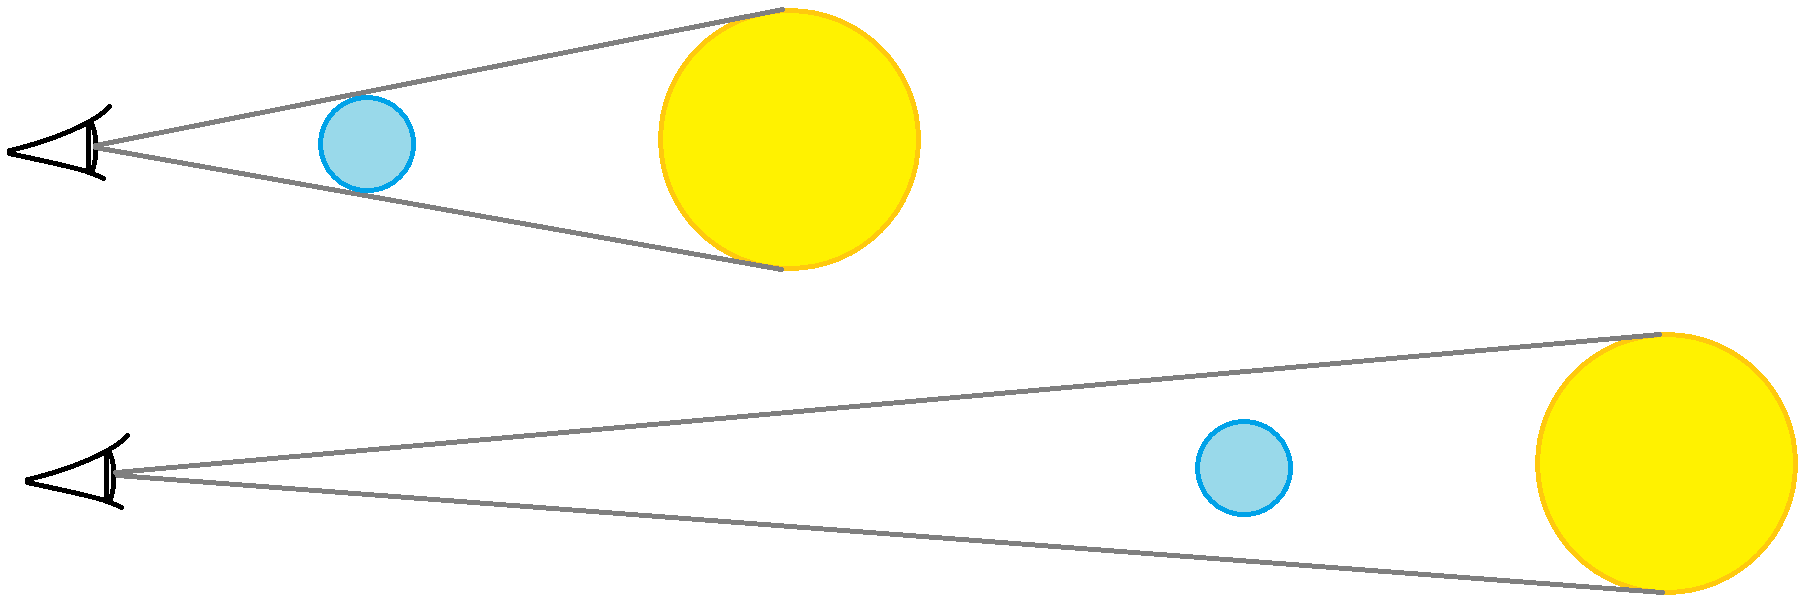
\includegraphics[width = 0.8\textwidth]{Astrofysik/billeder/UbetydeligRadius.png} 
    \caption{Illustration af at jo længere man er fra stjernen, des mindre afgørende er exoplanetens afstand til sin stjerne for hvor meget af lyset den dækker}
    \label{UbetydeligRadius} %misvisende navn
\end{figure}

Dette medfører også at planetens afstand til sin stjerne faktisk ikke har betydning for, hvor stor en formørkelse vi ser. Hvis lyset fra alle dele af stjernen flyver parallelt for at ramme os, så handler det kun om, hvor stor radius planeten har i forhold til stjernen. Antaget at lyset fra planeten er tæt på 0, er dybden af passagen

%Indsæt formlen med radier
\begin{align} \label{eq:DeltaL}
    \frac{\Delta L}{L_\star } = \left( \frac{R_p}{R_\star } \right)^2
    %F_{total} = F_\star  + F_p = \frac{I_\star }{}
\end{align}

Luminositeten af stjernen $L_\star $ kan vi nemt finde, da den hænger sammen med hvordan dens spektrum ser ud. $\Delta L$ er hvor meget lysstyrken falder under et transit, $R_p$ er planetens radius og $R_\star$ er stjernens radius. Så hvis vi kender stjernens egenskaber og måler dybdet af transittet, er planetens radius den eneste ubekendte, som vi derfor kan isolere i ligningen og beregne.
%
Metoden er selvfølgelig begrænset af, at stjernesystemet skal have en vinkel i forhold til os, hvor planetens bane krydser stjernen. Planeter der ikke opfylder dette, må vi detektere med andre metoder.
%
Fra Jorden kan vi måle fluxen fra en stjerne, så ved at gøre dette over tid, kan vi se om der er variationer, som indikerer tilstedeværelsen af en eller flere planeter. Man plotter en lyskurve med flux eller luminositet (ved at korrigere fluxen for afstanden) som funktion af tid, og ser efter mønstre i dette, som på figur \ref{transit}.
%
\begin{figure}
    \centering
    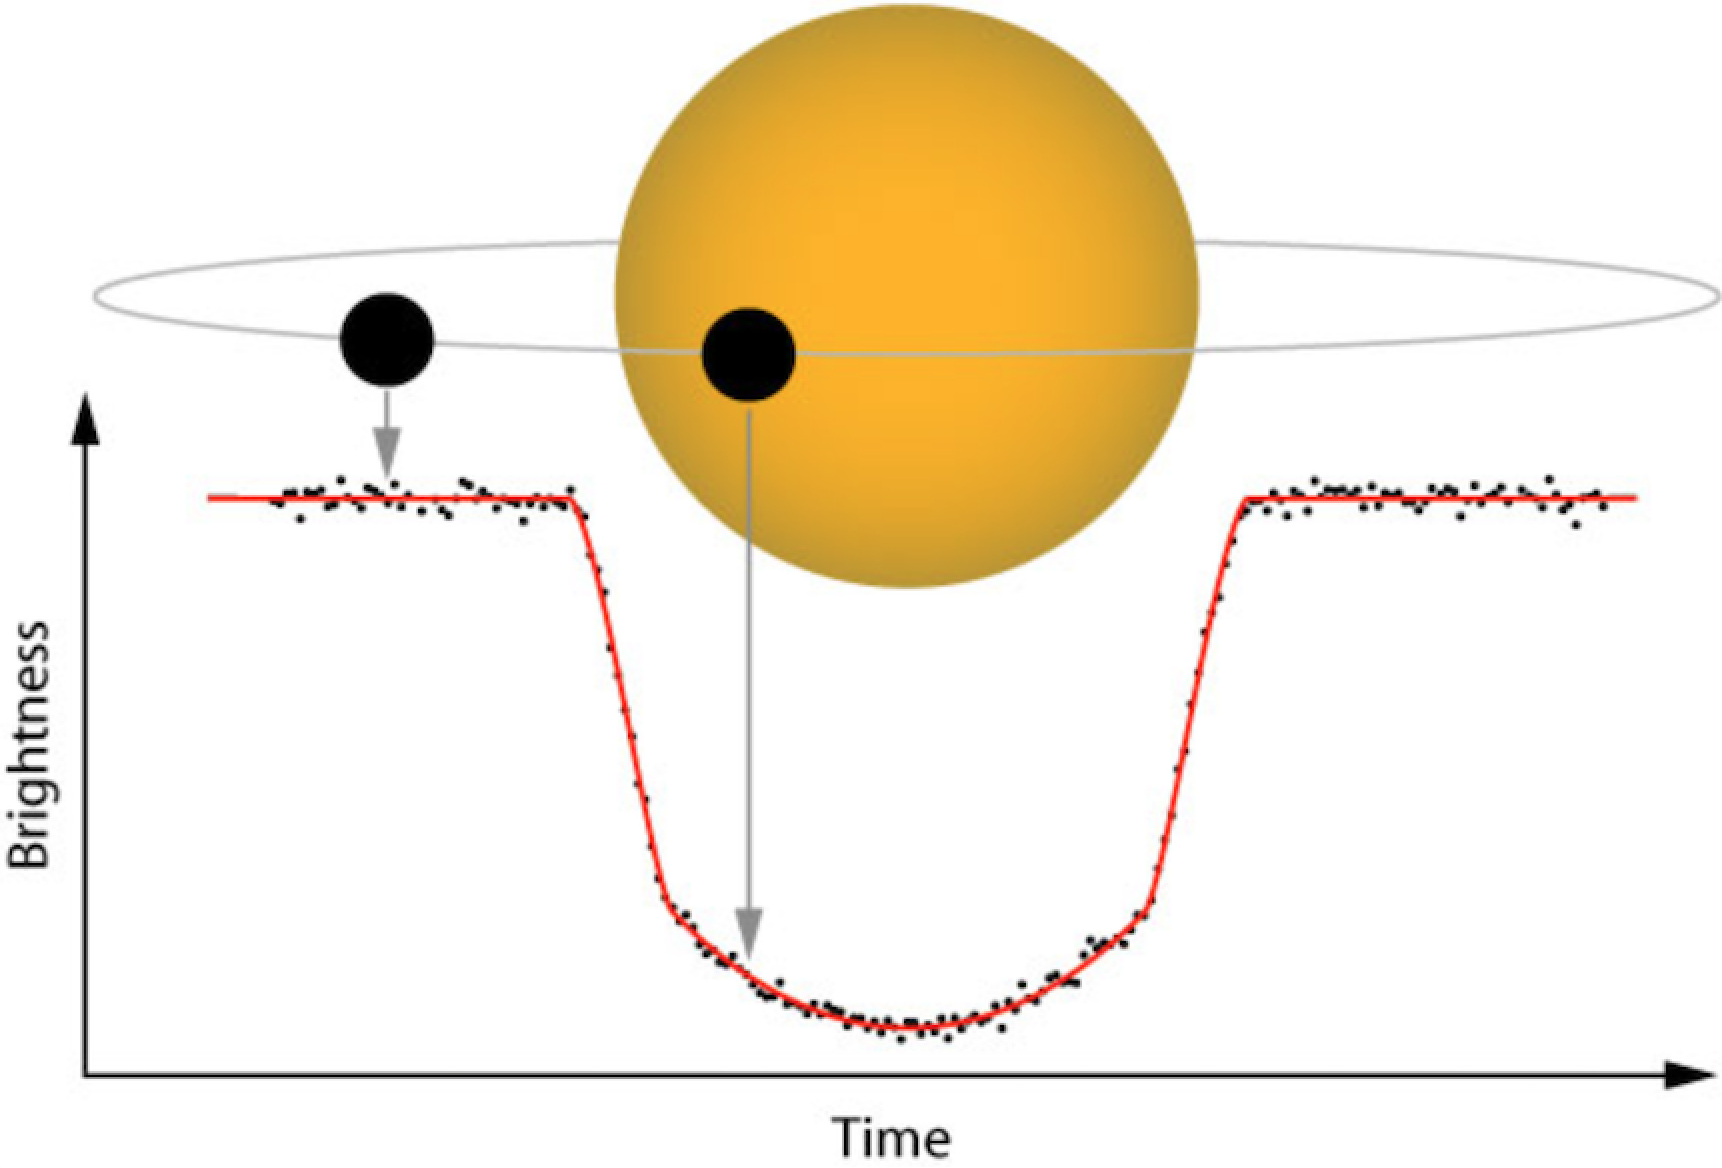
\includegraphics[width = 0.5\textwidth]{Astrofysik/billeder/transit.png}  
    \caption{Som planeten bevæger sig ind foran stjernen, skærmer den for mere af dens lys. På grafen vises luminositet som funktion af tid.}
    \label{transit}
\end{figure}
%
Når planeten først passerer ind over stjernen, ser vi et stejlt fald i lyskurven. Hældningen afhænger af planetens radius, da det for en stor planet vil tage længere tid før hele planeten er inde over stjernen. 
%
Derefter får vi en buet form i bunden af lyskurven, fordi stjernen lyser kraftigere i midten end ude i siden. Når planeten dækker stjernens midte, dækker den derfor en større andel af stjernens totale lys, end den ville, hvis den var ude i kanten af stjernen.
Når planeten passerer væk fra stjernen igen, ser vi det modsatte mønster. \\

Det er dog ikke det eneste interessante tidsrum. Når planeten ikke er ved at formørke stjernen, vil den nemlig stadig sende noget af dens lys i retning mod Jorden, og dermed øge lysstyrken. %\footnote{Planten reflekterer og udsender selvfølgelig hele tiden lys, men spørgsmålet er bare om det kan ses på Jorden. Hvis planeten er imellem dens stjerne og Jorden, vil planeten reflektere lys tilbage imod stjernen og altså væk fra Jorden.} 
Dette sker langsomt mens planeten bevæger sig om mod bagsiden af stjernen, hvor mere af mere af dens lys vil reflekteres - ligesom Månens faser ændrer sig som man nærmer sig fuldmåne. Men når planeten er direkte bag stjernen, får vi en planetformørkelse, hvor stjernen blokerer for lyset fra planeten, så der falder lyskurven til det niveau, der kun er genereret af stjernen selv. Dette kaldes det sekundære transit.
%
På figur \ref{fuld_lyskurve} ses en fuld lyskurve. Tidsaksen er elliptisk, så den følger hvordan planeten bevæger sig set fra Jorden. De stiplede linjer viser, hvordan fluxen ville være, hvis planeten og stjernen ikke påvirkede hinanden, mens den solide linje angiver den reelle lyskurve. Bemærk at selv natsiden af planeten vil bidrage med en smule lys. %Det kan fx skyldes refleksioner i atmosfæren og lys fra planeten selv.

\begin{figure}[h!]
    \centering
    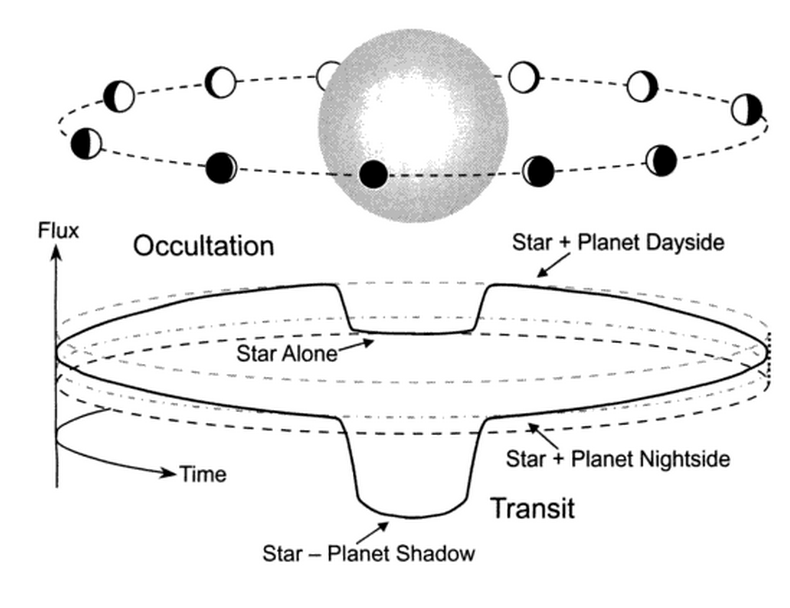
\includegraphics[width = 0.8\textwidth]{Astrofysik/billeder/fuld_lyskurve.png}  
    \caption{Lyskurven for et helt kredsløb med både primært og sekundært transit. Bemærk at tidensaksen er elliptisk, og fluxen er konstant hvis man holder en konstant højde over tidsaksen. \emph{Kilde: Aldaron, https://commons.wikimedia.org/w/index.php?curid=7274700}}
    \label{fuld_lyskurve}
\end{figure}

Ud fra transitmetoden kan man få mange oplysninger om planeten og dens stjernesystem:
\begin{itemize}
    \item \textbf{Planetens radius} kan fås fra hvor stor en del af stjernens lys der dækkes, men hænger også sammen med hældningen på lyskurven mens hele planetens overflade ikke dækker stjernen. Beregnet fra transittets dybde i enheder af stjernens luminositet $\frac{\Delta L}{L_\star }$ får man
    \begin{align}
        R_p = R_\star  \sqrt{\frac{\Delta L}{L_\star }}
    \end{align}
    \item \textbf{Inklinationsvinklen}, som er planetbanens hældning i forhold til os, kan vi også finde. Hvis planeten passerer ude i kanten af stjernen vil passagen nemlig tage kortere tid og lyskurvens form ændres.
    \item \textbf{Perioden} (dvs. årets længde for planeten) samt planetens \textbf{afstand} til stjernen hænger sammen ifølge Keplers 3. lov, hvis man kan estimere massen af systemet. De kan bestemmes ved at vente og se, hvornår dykket i lysstyrken vender tilbage, som følge af at planeten har været hele vejen rundt. Det øger desuden sikkerheden af, at vi virkelig har fundet en planet, jo flere gange signalet vender tilbage, da dyk i intensitet kan skyldes mange andre ting også. % + mange andre ting. "impact parameter", or how close to the center of the star the planet transits, the size of the star (or more precisely, how dense the star is), and the eccentricity of the planet's orbit, or how close to a circle the planet's orbit is"
    \item \textbf{Temperaturen} af planeten kan fås gennem det sekundære transit. Når planeten er i sekundært transit, måler vi kun stjernens lys og kan finde dens spektrum. Når planeten så er lige ved siden af stjernen og reflekterer mest muligt, kan vi tage et spektrum, som vil være summen af spektret fra planeten og det fra stjernen. Ved så at trække stjernens spektrum fra, får vi planetens spektrum. Hvor meget lys vi får fra den, kan afsløre dens temperatur.
    \item \textbf{Atmosfæresammensætningen} er rigtig interessant, hvis vi vil vide om der er liv på planeten, da fx oxygen er en god biomarkør. Den kan vi både se gennem planetens spektrum fra det sekundære transit, og gennem hvordan noget af stjernens lys kan blive absorberet under det primære transit. Her vil en del af det nemlig passere igennem atmosfæren. Dette uddybes i afsnit \ref{sec:liv}.
    \item \textbf{Solpletter} på stjernen kan også måles. Hvis planeten passerer henover en solplet, vil den kortvarigt skærme for en mindre del af stjernens lys, så der kommer et bump opad på lyskurven.
    \item \textbf{Planetens rotation} i forhold til stjernen kan bestemmes ved at se på ,hvornår hvilke dele af spektret blokeres. Dette vil vi ikke komme nærmere ind på her, men det kaldes Rossiter-McLaughlin-effekten og viser overraskende at, op til 25 \% af planeter af typen "Hot Jupitors" drejer modsat deres stjerne. 
    \end{itemize}
    
Endvidere kan man opdage ekstra planeter indirekte, hvis man ser at transitplaneterne opfører sig, som om en ekstra planet hiver i dem. Vi kan altså opnå utrolig meget viden ud fra det lys, vi modtager fra et stjernesystem, og vi ser, at karakteriseringen af exoplaneter er meget afhængigt af vores forståelse af stjerner.

\subsection*{Radialhastighedsmetoden}
Radialhastighedsmetoden er en anden effektiv metode. Radialhastighed er den del af en hastighedsvektor der peger mod observatøren, også kaldet den radielle komponent, som illustreret på figur \ref{radvel}. Det er derfor et mål for, hvor meget noget bevæger i vores retning. Hvor hurtigt det kommer tættere på eller længere væk fra os, selv hvis det i virkeligheden ikke bevæger sig direkte mod os. Grunden til at vi bruger radialhastigheden er, at den er nem at måle, og fra den kan man opnå information om:

\begin{figure}[h!]
    \centering
    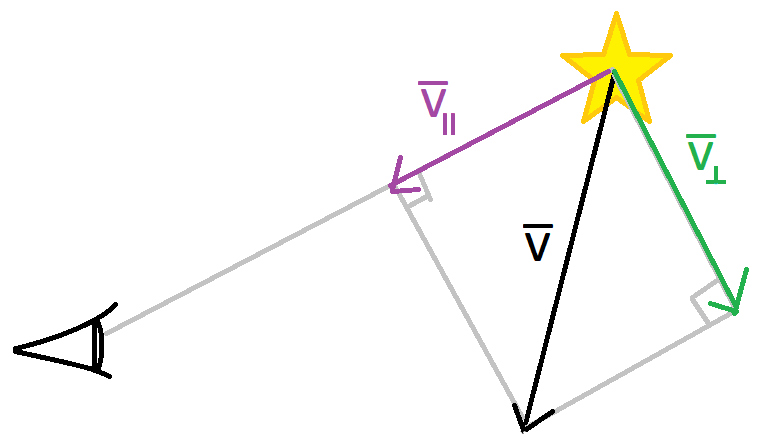
\includegraphics[width = 0.6\textwidth]{Astrofysik/billeder/radvel.png}  
    \caption{Illustration af en stjernes hastighed i forhold til en observatør. Den sorte pil angiver den totale hastighed, den grønne er den tangentielle hastighed, og den lilla er den radielle hastighed.}
    \label{radvel}
\end{figure}

\begin{itemize}
    %\item \textbf{Kraften} mellem stjernen og planeten fra Dopplerskiftet. %, hvilket er navnet på det fænomen at bølgers egenskaber påvirkes at kildens bevægelse. Dette er grunden til at lyden af et udrykningskøretøj ændres når det bevæger sig forbi en i trafikken.  %how % Dette har vi nu skrevet tidligere.
    \item \textbf{Perioden} hænger sammen med hvor ofte Dopplerforskydningen svinger mellem rødforskydning og blåforskydning. %Og perioden kan give os \textbf{afstanden} til stjernen gennem Keplers 3. lov.
    \item \textbf{Den radielle hastighed} af stjernen og planeten i deres fælles kredsløb kan godt findes, men den totale hastighed kræver andre metoder.
    \item \textbf{Massen} kan bestemmes, hvis vi kender stjernens masse, periode og radielle hastighed.
    %afstanden $r$ mellem stjernen og planeten og stjernens masse $M_\star$. $r$ og masserne $M_p$ og $M_\star$ hænger nemlig sammen ifølge Newtons tyngdelov. 
    Det er dog $M_p \sin(i)$ man finder, så uden at kende inklinationsvinklen $i$ har man kun en nedre grænse, da $\sin(i)$ kan være mellem 0 og 1. Men det plejer at passe inden for en faktor 2.  
    %\begin{align} \label{eq:FgNewton}
    %    F_g = G \frac{M_\star M_p}{r^2}
    %\end{align}
    \item \textbf{Densitet} kan man beregne ud fra massen og radius ved $\rho = \frac{M}{4/3 \pi R^3}$, hvis vi også kender radius fra at have observeret planeten med transitmetoden. Denne densitet er et gennemsnit over hele planeten, der her er antaget sfærisk.
    \item \textbf{Materialet} kan bestemmes fra densiteten. Dette gøres meget groft, men nogle materialer sætter øvre og nedre grænser på densiteten, og vi kan sammenligne med kendte planeter med lignende densiteter.
\end{itemize}

Radialhastighedsmetoden udnytter at planeten har masse, hvorfor både stjernen og planeten bevæger sig om et fælles massemidtpunkt. Eftersom stjernen er meget tungere end planeten, vil det resultere i at planeten bevæger sig meget mere end stjernen, og massemidtpunktet kan befinde sig inde i stjernen. Dette kan ses ud fra vægtstangsprincippet
\begin{align} \label{vstang}
    M_pr_p = M_\star r_\star 
\end{align}
hvor $M_p$ og $r_p$ er hhv. planetens masse og afstand til stjernen og planetens fælles massemidtpunkt, og ligeså for stjernen. For kontekstens skyld kan vores Solsystem nogenlunde approksimeres til kun at bestå af Solen og Jupiter, hvorfor afstanden fra Solens centrum til solsystemets massemidtpunkt, i solradier, er
\begin{align}
    r_\odot = \frac{M_\textit{\textsc{j}}r_\textit{\textsc{j}}}{M_\odot} = \SI{1.07}{R_\odot} \, ,
\end{align}
hvor subscriptet $\odot$ indikerer, at det er en af Solens egenskaber.\footnote{Jorden kan tilsvarende angives ved subscriptet $\oplus$.} Det ses altså, at Solen roterer om et punkt lidt uden for dens overflade, og det kan derfor konkluderes at Solen bevæger sig, men ikke ret meget ift. planeterne omkring den.\\

Stjernens bevægelse kan dog være nok til, at det kan ses fra Jorden. Vi har svært ved at observere stjernens bevægelse i andre retninger en den radielle, så stjernen ser ud som om den svinger skiftevis mod os og væk fra os. Lys er elektromagnetiske bølger og påvirkes derfor af Dopplerforskydning som beskrevet i sektion \ref{exointro}.
%lidt groft sagt kan det siges at når stjernen bevæger sig mod os, så skubber den bølgen sammen, hvorved bølgelængden bliver kortere og modsat når den bevæger sig væk fra os. Denne forskydning af bølgelængde som følge af kildens hastighed kaldes en Dopplerforskydning eller rød-/blåforskydning i astronomi, hvor farven angiver retningen.
%Da rød svarer til lange bølgelængder og blå til korte (indenfor det synlige spektrum), så refererer rødforskydning til noget som bevæger sig væk fra os og vice versa. Dette virker fordi en lyskildes spektrum afhænger meget distinkt af hvor lyset kommer fra og hvad det har skulle bevæge sig igennem for at nå til jorden. Stjerners overflader består af forskellige grundstoffer og forskellen mellem to energiniveauer i hvert grundstof svarer til en hel bestemt bølgelængde. Da der er mange mulige overgange for hvert atom kan det identificeres ud fra de spektrallinjer, atomet skaber i spektret, altså hvilke bølgelængder, der absorberes af atomet. 
Dopplereffekten gør det at hele spektret flyttes, og det betyder at stjernes hastighed kan bestemmes ved at finde ud af, hvor meget spektret skal "flyttes" for at spektrallinjerne falder tilbage til den form det ville have, hvis det ikke var blevet Dopplerforskudt.

\begin{figure}[h!]
    \centering
    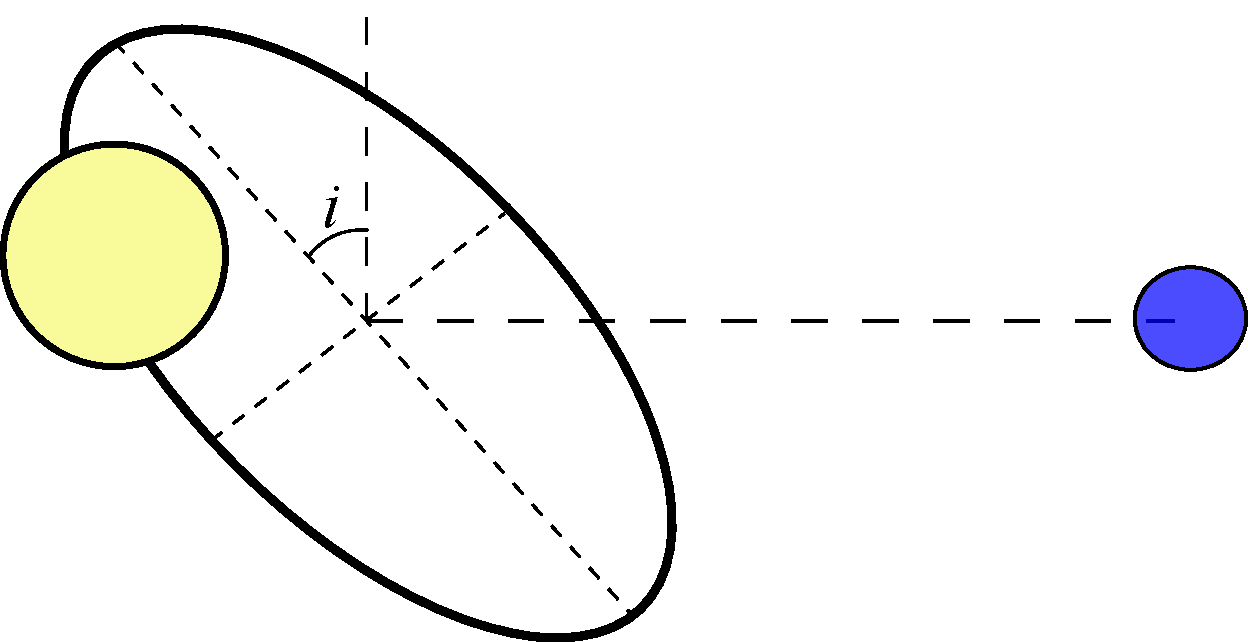
\includegraphics[width=.7\textwidth]{Astrofysik/billeder/Inklinitionsvinkel.pdf}
    \caption{Stærkt fortegnet illustration af situationen for radialhastighedsmetoden. Den hastighed vi kan bestemme på Jorden ud fra Dopplerforskydningen er en radielle bevægelse i samme plan som vi ser stjernen, dvs. langs med den stiplede linje fra Jorden. Stjernen kan dog også bevæge sig i de to andre dimensioner, som ikke kan "ses" fra Jorden. Den samlede fart afhænger derfor af inklinationsvinklen $i$, som er vinklen mellem den plan stjernen bevæger sig i og synslinjen til stjernen fra Jorden.} %Og en faktor mere, right? Det kan jo være elliptisk
    \label{fig:vsini}
\end{figure}

\subsubsection{Estimat af planetens masse fra radialhastighedsmetoden}
Planetens masse og afstand til sin stjerne er helt essentielle parametre, så dem vil vi forsøge at bestemme med udgangspunkt i Keplers 3. lov for to-legemesystemets fælles bevægelse
\begin{align} \label{kepler3lov}
    \frac{P^2}{r^3} = \frac{4\pi^2}{G(M_p+M_\star )}
\end{align}
hvor $P$ er stjernen og planetens fælles periode, $G$ er Newtons gravitationskonstant, $r$ er afstanden mellem dem, og det kan også udtrykkes som summen af afstandenene fra hhv. stjernen og planeten til deres fælles massemidtpunkt. Antager vi nu, at både planeten og stjernen er i jævn cirkelbevægelse omkring deres fælles massemidtpunkt, kan vi anvende ligning \ref{vstang} og få
\begin{align}
    r = r_\star+r_p  = r_\star  + \frac{M_\star r_\star }{M_p}
\end{align}
Det er dog afstanden i tredje, der skal bruges til Keplers 3. lov, som så det opskriver vi
\begin{align} \label{rvstang}
    r^3 = r_\star ^3\left(1 + \frac{M_\star }{M_p}\right)^3 = r_\star ^3\left(\frac{M_\star  + M_p}{M_p}\right)^3
\end{align}
Antagelsen om jævn cirkelbevægelse er nødvendig for at opnå et simpelt udtryk for planetens masse, selvom den ikke altid er lige god, men dog tilstrækkelig til at få en idé om størrelsen.\footnote{Det er en generel ting i fysik at jo mere præcist vi forsøget at beskrive verden desto mere kompliceret bliver det, og at vi derfor hurtigt bliver nødt til at approksimere, hvilket specielt ses i kapitlerne om analytisk mekanik og atom- og molekylefysik.} \\
Perioden er den tid det tager et objekt at bevæge sig en hel omgang om sit rotationspunkt, hvilket også kan udtrykkes som forholdet mellem den tilbagelagte afstand og hastigheden. For stjernen bliver det derfor (antaget cirkelbevægelse)
\begin{align}
    P_\star  = \frac{2\pi r_\star }{v} \label{Pstar}
    %P_\star  = \frac{2\pi r_\star }{v_\star ^\mathrm{rad}} \label{Pstar}
\end{align}
hvor $v$ er stjernens samlede fart. Problemet er bare, at med Dopplerforskydning kan vi kun se farten parallelt med vores synslinje dvs. den radielle hastighed $v_{||}$. Hvis stjernen ikke roterer i samme plan som vi ser den fra, er der en hastighedskomponent vi ikke får målt, se figur \ref{fig:vsini}. Fra denne figur ses det, at vi vha. trigonometri kan udtrykke den observerede hastighed $v_{||}$ som

%hvor $||$ er et superscript, der indikerer at der er tale om en radiel hastighed parallel med vores synslinje. Radialhastighedsmetoden er jo netop, at vi kan bestemme den radielle fart, $v_{||}$, ud fra spektroskopi (at kigge på spektrallinjer). Problemet er bare, at stjernen ikke nødvendigvis roterer i det plan vi ser den fra, se figur \ref{fig:vsini}. Fra denne figur ses det, at vi kan udtrykke den observerede hastighed $v_{||}$ vha. trigonometri.
\begin{align}
    v_{||} = v \sin(i) \, ,
    %\tilde{v} = v_{*,\,\mathrm{obs}}^\mathrm{rad} = v_\star ^\mathrm{rad}\sin(i)
\end{align}
hvor $i$ er inklinationsvinklen og $v$ er stjernens samlede fart. Herfra skiftes notationen, som indikeret ved det første lighedstegn ovenfor, da det er simplere at skrive. %da det er til at blive idiot af symbolet $v_{*,\,\mathrm{obs}}^\mathrm{rad}$, selvom det fortæller præcist hvad det betyder. 
Herved bliver perioden
\begin{align}
    P_\star  = \frac{2\pi r_\star \sin(i)}{v_{||}} 
\end{align}
Kombineres dette med Keplers 3. lov (ligning \eqref{kepler3lov}) fås
\begin{align}
    \frac{4\pi^2}{G(M_p+M_\star )} = \frac{P_\star ^2}{r ^3} = \frac{P_\star ^3}{P_\star r ^3} = P_\star ^3 (P_\star r ^3)^{-1} = \left(\frac{2\pi r_\star \sin(i)}{v_{||}}\right)^3\left(P_\star r^3\right)^{-1}
\end{align}
Tricket med at forlænge brøken med perioden kan virke uintuitivt, men det tillader os at benytte ligning \eqref{rvstang} således
\begin{equation}
\begin{aligned}
    \frac{1}{G} &= 2\pi\sin^3(i)\left[v_{||}^3P_\star \dfrac{(M_\star +M_p)^2}{M_p^3}\right]^{-1} \\
    \implies M_p^3\sin^3i &= \frac{P_\star v_{||}^3(M_\star +M_p)^2}{2\pi G}
\end{aligned}
\end{equation}
Det virker som om der sker en hel masse her, men i virkeligheden er der ikke sket andet, end indsættelsen af ligning \refeq{rvstang} og en efterfølgende reduktion af ligningen til en nogenlunde pæn form. Dette opfordres læseren til at tjekke efter. \\
Stjernen vil ofte være meget tungere end planeten, hvorfor kan være en rimelig antagelse, at summen af de to masser bare er stjernens masse, $M_\star  + M_p\approx M_\star $, hvorved følgende opnås
\begin{align}
    M_p\sin(i) \approx v_{||}\left(\frac{P_\star M_\star ^2}{2\pi G}\right)^{1/3}
\end{align}
Da udtrykket afhænger af $i$, kræver dette, at $i$ kan bestemmes på andre måder. Det er en klar svaghed ved metoden, da $i$ kan være svær at bestemme. Men man får en nedre grænse for massen. Derudover er radialhastighedsmetoden selektiv over for tunge planeter på tæt stjernen, da $v_{||}$ må være stor nok til at vi kan se, hvordan den trækker i stjernen.

\subsection*{Astrometri}
Udfordringen ved radialhastighedsmetoden er, at vi netop kun måler den radielle komponent af hastigheden, og ikke kender den fulde version. For at metoden kan virke optimalt, skal $\sin(i)$ helst være så stor som muligt, da Dopplerforskydningen så er størst (og man får et størst muligt minimum for massen). Er $\sin(i)$ meget lille, svarer det til at se systemet enten oppefra eller nedefra. Så bliver Dopplerforskydningen relativt lille, og radialhastighedsmetoden bliver svær at bruge. Men planeten vil stadig hive i stjernen langs andre akser - vinkelret på vores synsfelt. Teknisk set kan denne bevægelse ses, og kan dette gøres konsistent nok, er det muligt at bruge det til at detektere planeten i bane om stjernen. Stjerner er dog så langt væk, at selvom de bevæger sig meget, så ser bevægelsen lille ud herfra, og det kræver meget store teleskoper med meget god opløsning. \\

Med astrometri kan vi opnå information om %observere parametre omkring stjernen og planetens indbyrdes bevægelse, hvorfor der kan opnås information om
\begin{itemize}
    \item \textbf{Inklinationsvinklen} af systemet.
    \item \textbf{Massen} kan bestemmes, lidt parallelt til hvordan det gøres for radialhastighedsmetoden.
    \item Kan inklinationsvinklen bestemmes, samtidig med at der er data, som kan bruges til radialhastighedsmetoden, bliver det muligt at bruge denne til at bestemme fx massen med høj præcision.
    \item I kombination med direkte observation af planeten kan planetens banebevægelse beskrives med høj præcision.
\end{itemize}

\begin{figure}[h!]
    \centering
    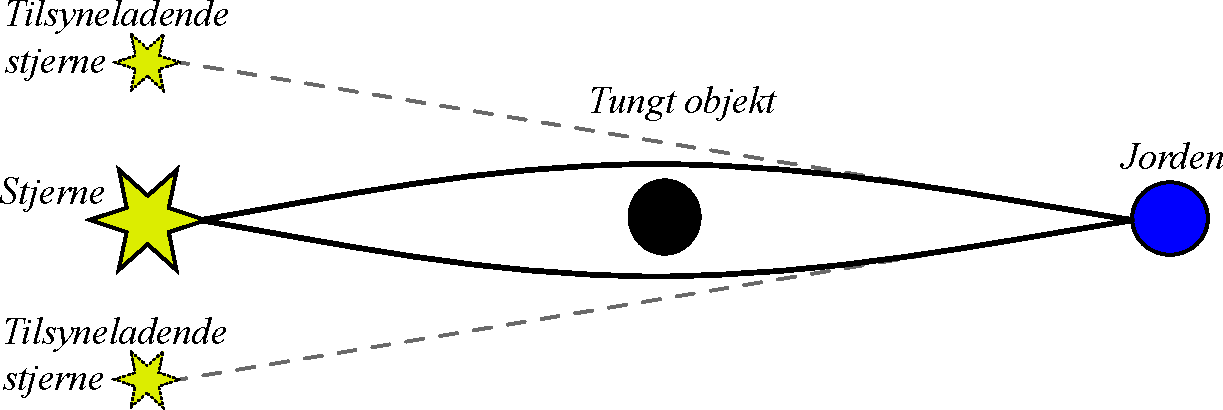
\includegraphics[width=\textwidth]{Astrofysik/billeder/GravLinse.pdf}
    \caption{Lys udsendt fra en fjerntliggende lyskilde afbøjes af tyngdefeltet fra objektet i midten. Som de grå stiplede linjer indikerer ser det ud til at der skulle være to mindre identiske stjerner, frem for én større, når de ses på Jorden.}
    \label{fig:GravLinse}
\end{figure}

%Liste med egenskaber man kan finde
\subsection*{Gravitationslinsemetoden} \label{sec:GravLinse}
Klassisk set er lys masseløse elektromagnetiske bølger, hvorfor det ikke påvirkes af tyngdekraften. Det falder dog ud af den specielle relativitetsteori, at energi og masse er to sider af samme sag, og da lys har energi, så påvirkes det også af tyngdekraften. Det bevæger sig stadig i lige linjer, men vil se bøjet ud, fordi tyngdekraften ændrer på, hvad en lige linje er - det får selve rummet til at krumme, som beskrevet i generel relativitetsteori. Denne effekt er dog lille nok til, at den klassiske beskrivelse holder i mange situationer, hvorfor den klassiske beskrivelse ikke altid bør forkastes. Astrofysiske objekter kan dog være så tunge, at effekter af rumtidens krumning observeres. Dette ses blandt andet ved eksistensen af det, som kaldes \textit{gravitationelle linser}. En linse spreder eller fokuserer lys, hvilket uddybes i kapitel \ref{cha:Optik}. En gravitationel linse virker essentielt set på samme måde, som en almindelig konveks linse, da gravitation kun er tiltrækkende.\footnote{Dette gælder så længe negativ masse ikke er en ting, hvilket alt empiri peger mod.} I figur \ref{fig:GravLinse} ses en illustration af princippet i en gravitationel linse, hvor lyset fra den bagvedliggende kilde fokuseres omkring et tungt objekt. Det medfører at vi modtager mere lys, end hvis det midterste legeme ikke havde været der, og at lyskildens position på himlen bliver forskudt, forvrænget og måske splittet til flere versioner forskellige steder. Hvis objektet i midten bevæger sig, så ændres fluxen på Jorden sig markant. På denne måde kan tunge objekter, som ikke selv udsender nok lys, til at vi kan se dem, detekteres på Jorden. Hvis det midterste objekt er en stjerne med en tilhørende planet, vil der være et tidspunkt, hvor planetens position får fluxen fra den fjerne stjerne til i "kort"  tid at øges og falde igen. Så hvis man plotter fluxen på en lyskurve, vil det give et lille peak. Hvis dette peak kan karakteriseres ud fra flere målinger, og der er samme effekt alle stedet, så er det muligt at konkludere, at en ny planet er fundet. \\

Ud fra gravitationslinsemetoden, hvor det afbøjende objekt er et stjernesystem, kan man opnå information om
\begin{itemize}
    \item \textbf{Systemets masse} ved at se hvor forvrænget det bagvedliggende lys bliver. Hvis lyskilden danner en ring kan man fx måle dens størrelse. Man må tage højde for afstandene mellem lyskilden, stjernesystemet og Jorden, samt hvor langt objekterne er fra hinanden på himlen. Hvis lyskilden er næsten på samme synslinje fra Jorden som stjernesystemet, vil linseeffekten påvirke det mere.
    %\item \textbf{Einsteinringens størrelse} for stjernesystemet, der hænger sammen med systemets masse og de indbyrdes afstande mellem baggrundsstjernen, systemet der forårsager lensingen, og Jorden. Massen er dog den samlede masse, hvorfor den inkluderer både stjerne, planet og hvad der ellers skulle være i stjernesystemet.
    \item \textbf{Masseforholdet} mellem stjernen og planeten kan findes, ved at se hvor stor linseeffekten er, når planeten bidrager i forhold til når den ikke gør. Det medfører, at \textbf{planetens masse} kan bestemmes, forudsat at stjernens masse kan bestemmes på anden vis. Metoden er særligt interessant, fordi man med gravitationslinser kan se selv relativt små planeter på størrelse med Mars.
    \item \textbf{Afstanden} mellem baggrundskilden og stjernesystemet kan approksimeres, hvis området hvori de to objekter er, er relativt kendt. Har man en grov idé om, hvor de to befinder sig, kan man sammenligne deres relative bevægelse med, hvordan ting i de områder typisk bevæger sig, og på den måde komme frem til en indbyrdes afstand.
    %\item \textbf{Højsopløsningsdata} af exoplaneter, da man i dag har den teoretiske forståelse, til at benytte Solen som en gravitationel linse, der kan fokusere lys andre steder fra, og derved forbedre opløseligheden af målinger derfra. Man har endnu ikke den praktiske kunnen, men det er måske en mulighed i fremtiden. % Kilde: https://journals.aps.org/prd/abstract/10.1103/PhysRevD.96.024008#fulltext
    \item \textbf{Afstanden} fra planeten til stjernen kan ses, men kun ved et bestemt tidspunkt. %Perioden? Afstanden til stjernen?
\end{itemize}

En ulempe ved gravitationslinsemetoden er, at den den er afhængig af et objekt der passerer bagved stjernesystemet, og som sandsynligvis aldrig vender tilbage. Så man har kun kort tid til observationerne, og de kan ikke gentages.

Der kan desuden være en fremtid i at anvende Solen som gravitationel linse til at tage højopløsningdata fra fjerne objekter. Dette har vi dog ikke den praktiske kunnen til endnu.

% Kilde: http://spiff.rit.edu/classes/resceu/lectures/microlens/microlens.html

%\subsection*{Pulsartiming}


\begin{figure}[h!]
    \centering
    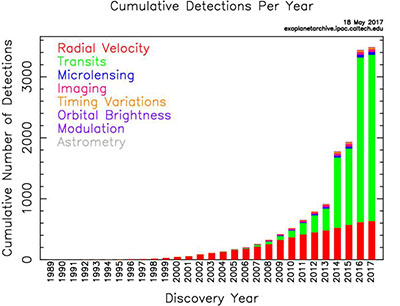
\includegraphics[width = 0.8\textwidth]{Astrofysik/billeder/AntalFundne.jpg}  
    \caption{Antal fundne exoplaneter efter årstal og sorteret efter metode. \textit{Kilde: NASA IPAC Exoplanet Science Institute}}
    \label{antal_fundne}
\end{figure}

\subsection*{Sammenligning}
Da der er så mange forskellige metoder at detektere exoplaneter med, er det værdifuldt at have et overblik over deres styrker og svageheder. Af figur \ref{antal_fundne} ses, at vi generelt bliver bedre til at finde exoplaneter, hvilket der kan være mange årsager til. Den mest oplagte er at instrumenter, teknologier og vores viden om exoplaneter forbedres. Det handler langt hen af vejen om at se små ændringer i det lys en stjerne udsender, sammenlignet med hvordan det ellers ville have set ud. Jordens atmosfære kan både sprede lys, absorbere dele af det og udsende mere, hvorfor det giver mere præcise målinger at benytte rumteleskoper for at undgå disse forstyrrelser. Så når vi får flere af disse, og dedikerer mere af deres tid til exoplaneter, vil vi også gøre flere opdagelser i feltet. Der er fx høje forventninger til James Webb Space Telescope, som med sin høje præcision måske vil kunne afgøre, om der er liv på andre planeter.  %Som flere missioner bliver iværksat gøres mere data tilgængeligt for forskere, hvorfor der er flere mulige stjerner at kigge på. 
Erfaringen fra tidligere missioner kan også forbedre de næste. Derudover må nogen jo betale for forskningen, og når først der er publicerede artikler, der viser at noget er muligt, og at det kan være interessant at undersøge noget, så bliver det lettere at skaffe penge til. \\ %Det er derfor ikke urealistisk at antage, at mængden af tid og penge, der bruges på at finde exoplaneter, er stigende. \\

Det ses også at radialhastighedsmetoden var dominerende i starten, indtil den i 2014 blev overhalet af transitmetoden i antal opdagede planeter. %En mulig årsag til dette kan være at transitmetoden måske kræver en højere præcision i målingerne af stjernens lys.
Keplersatelitten blev sat i kredsløb om Jorden i 2009 og har siden 2011 sendt data tilbage om tusindvis af exoplaneter, primært fundet vha. transitmetoden. %til Jorden om det galaktiske nabolag. Keplers tilstedeværelse giver bedre data, der gør det muligt at detektere flere exoplaneter. Som rumteleskob bliver Keplersatelitten ikke påvirket af Jordens atmosfære, som teleskoper nede på jorden, hvilket kan være afgørende for opdagelsen af exoplaneter. \\

Nogle detektionsmetoder er meget afhængige af, hvordan stjernen og planetens bevægelse er orienteret, ift. det plan hvori vi ser dem. Selvom en planet kan være kæmpestor og meget tæt på sin stjerne, så den hiver meget i stjernen, kan den være stort set usynlig for radialhastighedsmetoden, hvis $i\approx\SI{0}{\degree}$ eller $i\approx\SI{90}{\degree}$. Stjernen vil rigtig nok bevæge sig en hel masse, men ikke parallelt med synslinjen, så lyset ikke Dopplerforskydes meget. Denne planet ville dog være ideel til at detektere med astrometri, men med henvisning til figur \ref{antal_fundne} ses det, at astrometri ikke er nær så effektiv som radialhastighedsmetoden, hvorfor planeten måske overses. \\

\begin{figure}[h!]
    \centering
    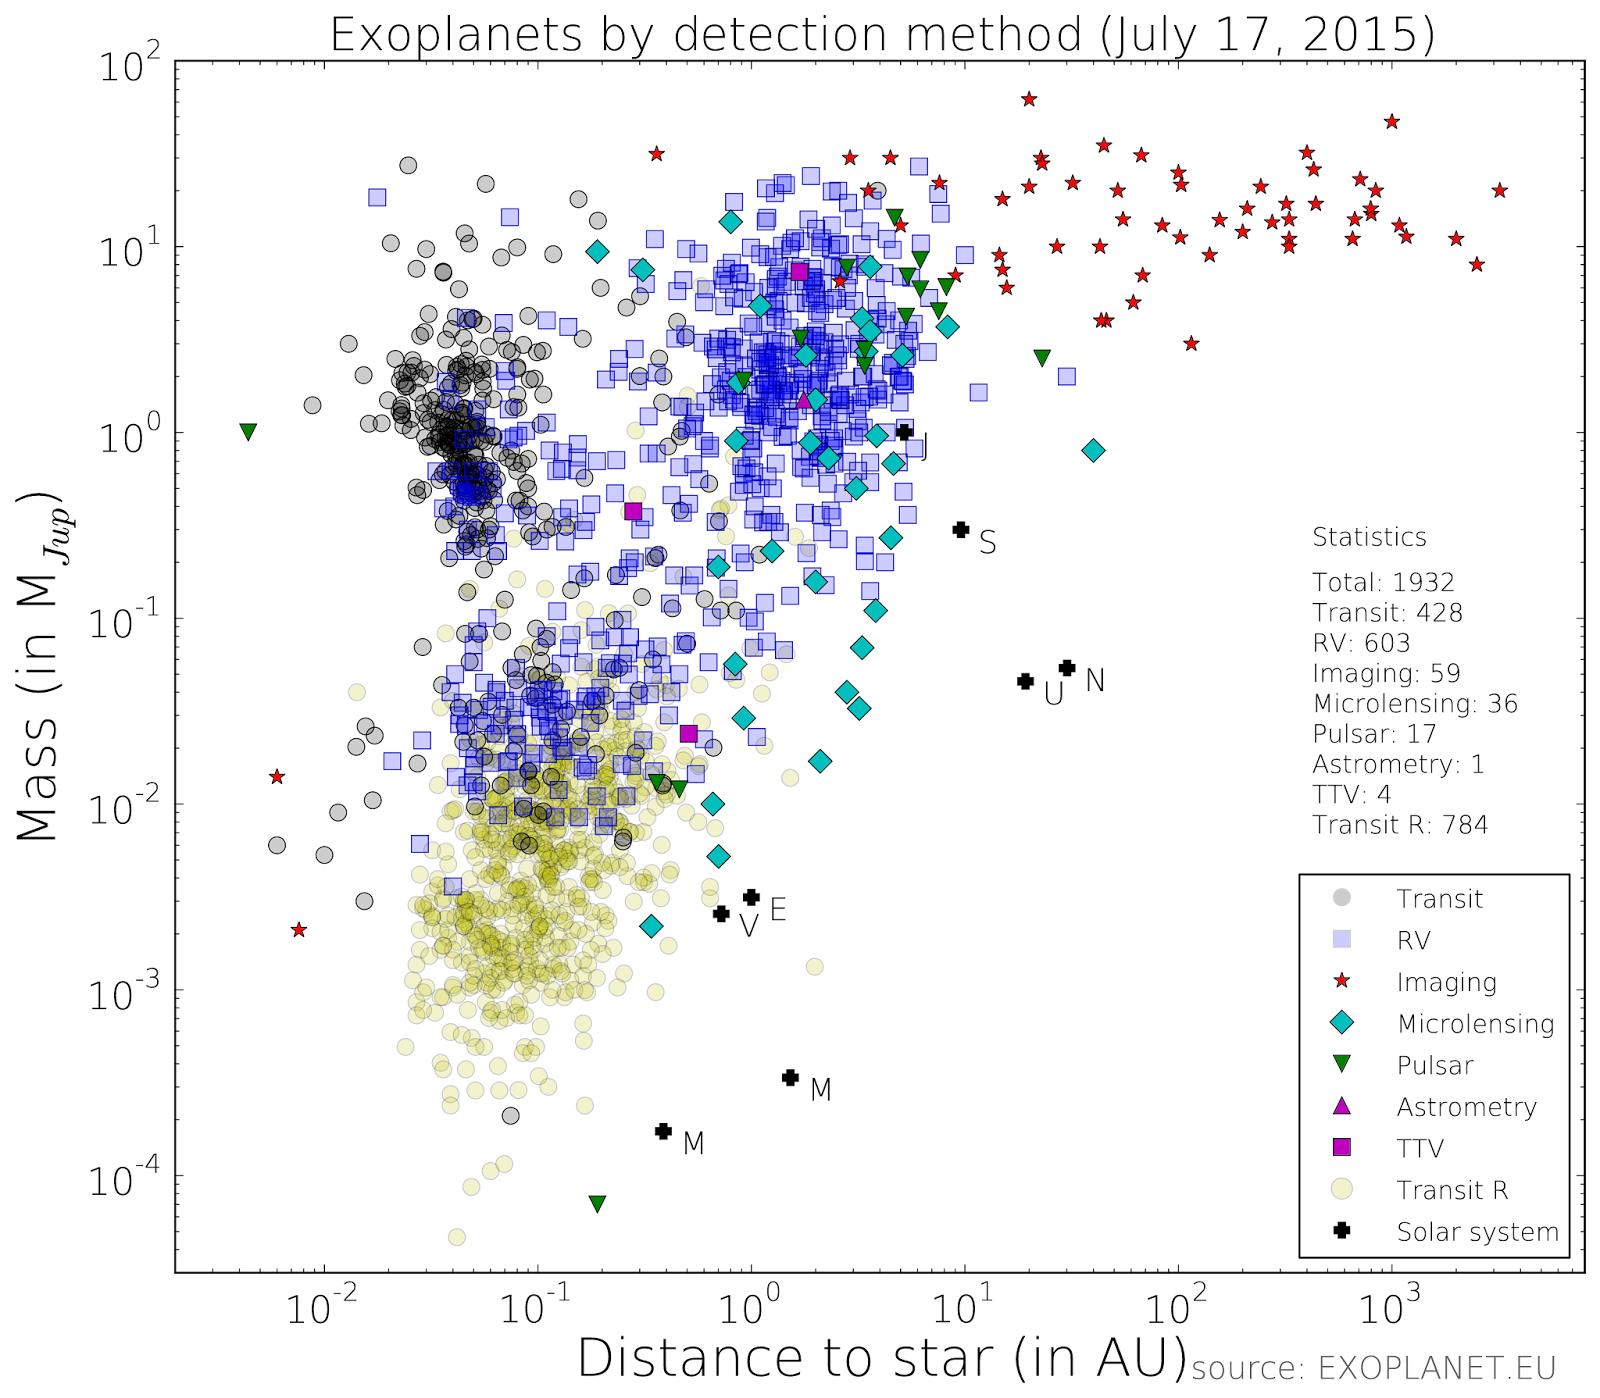
\includegraphics[width=.8\textwidth]{Astrofysik/billeder/sammenligning.PNG}
    \caption{Her ses de pr. 17. juli 2015 fundne exoplaneter, deres masse, afstand til den nærmeste stjerne, og den metode de er fundet ved. Yderligere er planeterne i Solsystemet indtegnet med sort. Det ses, at planeter meget langt fra deres stjerne kun er fundet ved direkte observation (dem fundet tæt på stjernen er formegentlig en fejl), samt at de andre metoder mest finder tunge planeter, tæt på deres stjerne. Bemærk de logaritmiske akser og enhederne - $M_{jup}$ er Jupitermasser og AU er Jordens afstand til Solen. \emph{Kilde: exoplanet-diagrams.blogspot.dk/2015/07/exoplanets-by-detection-method.html}}
    \label{fig:sammenligning}
\end{figure}

I afsnittet om transitmetoden fremgår det, at jo større planeten er relativt til stjernen, desto tydeligere vil den sænke systemets luminositet, se ligning \ref{eq:DeltaL}. Det betyder at en "stor" planet i bane om en "lille" stjerne vil være lettere at detektere på denne måde end den modsatte situation. Dette er et eksempel på en relativt generel tendens i detektionsmetoderne. De fleste favoriserer store planeter tæt på deres stjerne, da de så påvirker stjernen mest. Det er vigtigt, da det ofte er stjernens lys, og ikke planetens, der ses på Jorden, og planeten detekteres ved den måde den får stjernen til at bevæge sig på. Dette kan ses fra Newtons tyngdelov,
\begin{align} \label{eq:FgNewton}
    F_g = G \frac{M_\star M_p}{r^2},
\end{align}
hvor kraften er proportional med planetens masse over dens kvadrerede afstand til stjernen. Denne effekt finder sted ligeså snart stjernens bevægelse benyttes, hvorfor det ikke er aktuelt for eksempelvis direkte observation, men som det fremgår af afsnittet favoriserer denne metode også store, tunge planeter, dog via nogle andre argumenter. \\

I figur \ref{fig:sammenligning} ses et plot over kendte exoplaneter, deres masse, afstand til nærmeste stjerne samt den metode vi har fundet dem med. Ovenfor blev det konkluderet at tunge planeter tæt på deres stjerne, er favoriseret af de fleste detektionsmetoder. Dette ses ved de mange punkter øverste venstre hjørne på figuren, sammenlignet med at nederste højre hjørne er fuldstændig tomt - men der er også en faktor fra, at der nok blot findes færre små planeter langt fra deres stjerner.  Det skal også nævnes at planeter markeret som "Transit R", adskiller sig udelukkende fra "Transit", ved at massen er et kvalificeret gæt. Man har brugt planetens radius, antaget en densitet der er rimelig for planeter af dens størrelse, og derved estimeret massen. Det ses også tydeligt at radialhastighedsmetoden og transitmetoden er de klart mest effektive, samt at transitmetoden har den mest markante favorisering af planeter, som er tæt på. For at noget kan kaldes en planet, er det ikke nok at observere ét transit, så transitmetoden kræver at årets længde på planeten er kort nok - men perioden hænger sammen med afstanden til stjernen ifølge  Keplers 3. lov, ligning \ref{kepler3lov}, så det sætter en begrænsning på afstanden. Radialhastighedsmetoden favoriserer hovedsageligt tunge planeter, som kan være lidt længere væk.  %Keplers 3. lov, ligning \ref{kepler3lov}, giver at perioden er stor, hvis også afstanden til stjernen er stor, hvilket betyder at der går lang tid mellem transit, hvilket mindsker sandsynligheden for at observere det flere gange. \\
Det er også meget markant, hvordan direkte observationer skiller sig ud. Det er den eneste metode som har fundet de fjerne planeter, som i nogle tilfælde også ligger meget længere fra deres stjerne end Neptun gør fra Solen. De to små planeter, der er fundet med direkte observation, er der en risiko for at det er fejl,\footnote{\url{http://exoplanet-diagrams.blogspot.dk/2015/07/exoplanets-by-detection-method.html?m=1}} hvilket blot styrker konklusionen om, hvilke planeter direkte observation favoriserer. \\
Her er også plottet nogle planeter, der er fundet med metoder, der ikke er beskrevet her, men de er ikke essentielle for at forstå de generelle tendenser i plottet.

Det er ret markant som Solsystemets planeter stort set falder helt uden for den tendens, vi ser for fundne exoplaneter. Dette kan skyldes mange ting. En mulighed er, at Solsystemet er meget specielt, hvilket kunne reducere sandsynligheden for liv andre steder - for hvad nu hvis liv kræver specielle forhold, siden vi netop er i et usandsynligt system? En anden mulighed er, at Solsystemet bare er et af mange stjernesystemer, og at der intet specielt er ved det, men at vi ikke er i stand til at se tilsvarende planeter i andre stjernesystemet godt nok. Begge fortolkninger er plausible, men vi ved med sikkerhed at metoderne er biased, så helt repræsentative er de fundne planeter i hvert fald ikke.